\documentclass[a4paper, british]{article}

% \usepackage{authblk}
\usepackage[utf8]{inputenc}
\usepackage[T1]{fontenc}
\usepackage{babel}
% \usepackage[margin=2.5cm,a4paper]{geometry}
% \usepackage[skip=1em]{parskip}
\usepackage{lmodern} 
\usepackage{microtype}
\usepackage[
pdfauthor={Adam Menne},
pdftitle={Cardiac response to suboptimal ambient temperatures in Daphnia},
pdfsubject={},
pdfkeywords={}]{hyperref}
% \usepackage{xcolor}
\usepackage{graphicx}
\graphicspath{ {./figures/} }
% \usepackage{float}
% \usepackage{enumitem}
% \usepackage{tikz}
% \usepackage{pgfplots}
\usepackage{booktabs} %tables no vertical lines
% \usepackage{array}
\usepackage[noabbrev]{cleveref}
% \usepackage{fancyhdr} %headers and footers
% \usepackage{titlesec}
% \usepackage{tcolorbox} % framed text boxes
% \usepackage{mathtools, amssymb, amsthm}
% \usepackage{gensymb}
\usepackage{siunitx}
\usepackage{csquotes}
% \usepackage{lettrine} % initials
\usepackage[
backend=biber,
style=numeric,
sorting=none,
doi=true,
isbn=false
]{biblatex}
\addbibresource{citations.bib}

\setlength{\parskip}{1em}
\setlength{\parindent}{0em}
\linespread{1.3}



\title{Chemistry 264\\ Practical 1}
\date{Last editted on \today}
\author{Adam Menne\\ Stellenbosch University}

\begin{document}

\maketitle

% \begin{abstract}
% \noindent
% Daphnia provide a good model for studying the temperature-dependence of heartrate in poikilotherms. This is of importance due to the looming threat of global warming due to climate change, results from this study will be indicative of effects on a wide range of organisms, as well as effects on ecosystems. In this study we will validate the effects of suboptimal temperature on the heartrate of Daphnia.
% \end{abstract}

% \newpage

\section{Introduction}

The crustacean genus Daphnia falls under the Daphniidae family, apart of the Crustacea subphylum, and the Arthropoda phylum. They are a good subject for this study for two reasons: the carapace is highly translucent, and they have a large heart in proportion to body size. This allows the heart beat of Daphnia to be easily observed under magnification. Interestingly, heartrate is not dependant of the size of the specimen, although does differ between species.\cite{santosoCardiovascularPerformanceMeasurement2020}

Being ectothermic poikilotherms, their metabolic rate, and heartrate, are extremely temperature dependant. Daphnia cannot self-regulate their metabolic rate to a significant degree, and thus their fitness and survival are highly dependant on a suitable habitat.

\newpage

While this study only covers these effects on a single species, the results will be indicative of a far wider range of organisms, and will have wider reaching ecological consequences.

This research is of importance particularly in terms of climate change and thermal pollution on many organisms and at a larger scale, ecosystems.

Rises in global temperatures due to climate change will result in continuous thermal stress over multiple generations, the effects observed in Daphnia may occur in other similar poikilotherms.
This may have significant effect on aquatic ecosystem dynamics.\cite{khanEffectTemperatureWaterflea2008}

Daphnia are of significant importance to the ecosystems of freshwater systems(which are highly susceptible to temperature fluctuations). With higher temperatures the metabolic rate of poikilotherms increases. In the case of Daphnia this leads to higher particle uptake rates, an increase in growth rate(although as a consequence of higher metabolic rates, body size will ultimately decrease), and a decrease in survival time. Conversely,  a decrease in temperature, will lead to a decrease in metabolic rate, lower particle uptake rates , reduced growth rate, but lower metabolic costs cause greater body sizes. Ultimately these effects lead to the fact that above 26 \textcelsius{} the survival rates of Daphnia decrease greatly.\cite{mullerTemperaturedrivenResponseReversibility2018}

Daphnia that become acclimatised to higher and lower temperature can have significant changes to their protein expression. Notably cold-repressed proteins are enzymes involved in protein digestion. Cold-induced proteins affected were vitellogenin(important for the development of oocytes), and actin.\cite{schwerinAcclimatoryResponsesDaphnia2009}

Furthermore these wide range of effects are of particular significance considering that Daphnia form a vital part of freshwater food chains, being filter feeders, they mainly consume algae and form a significant part of the zooplankton diet of many fish.\cite{santosoCardiovascularPerformanceMeasurement2020}

\section{Results}

Mean value for all temperatures are shown in \cref{fig:mean}

The data gathered was not very consistent, as seen in \cref{fig:density} the data for all three temperatures have high variance. However considering the large sample size, the 95\% confidence interval for the mean is relatively small for all temperatures. From this, the validity of the analysis is fairly certain.

Values for standard deviation, standard error, and CLM, are presented in \cref{table:1}

\begin{figure}[htb]
    \centering
    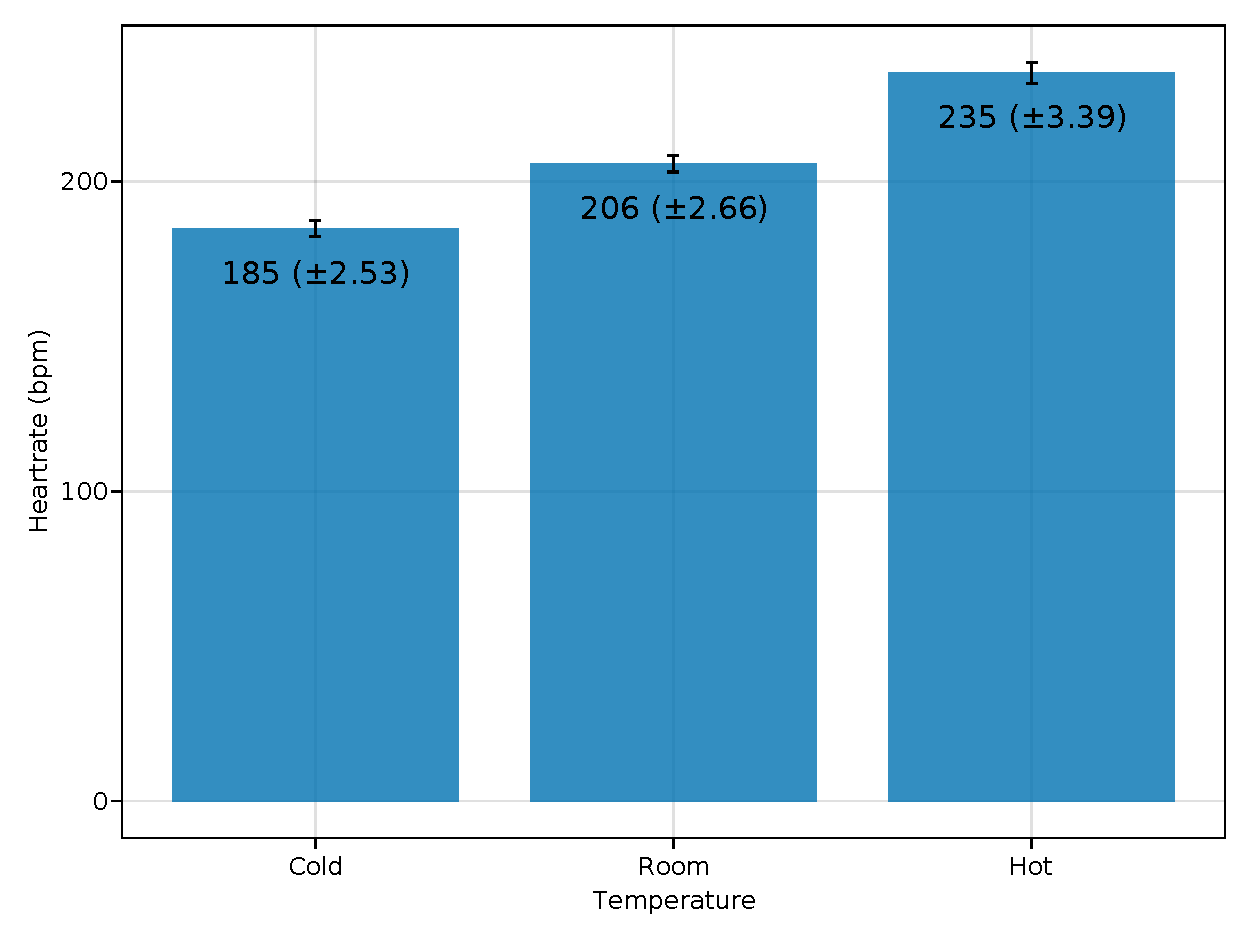
\includegraphics[width=0.75\textwidth]{figures/plot1.pdf}
    \caption{Mean temperatures with CLM}
    \label{fig:mean}
\end{figure}

\begin{figure}[htb]
    \centering
    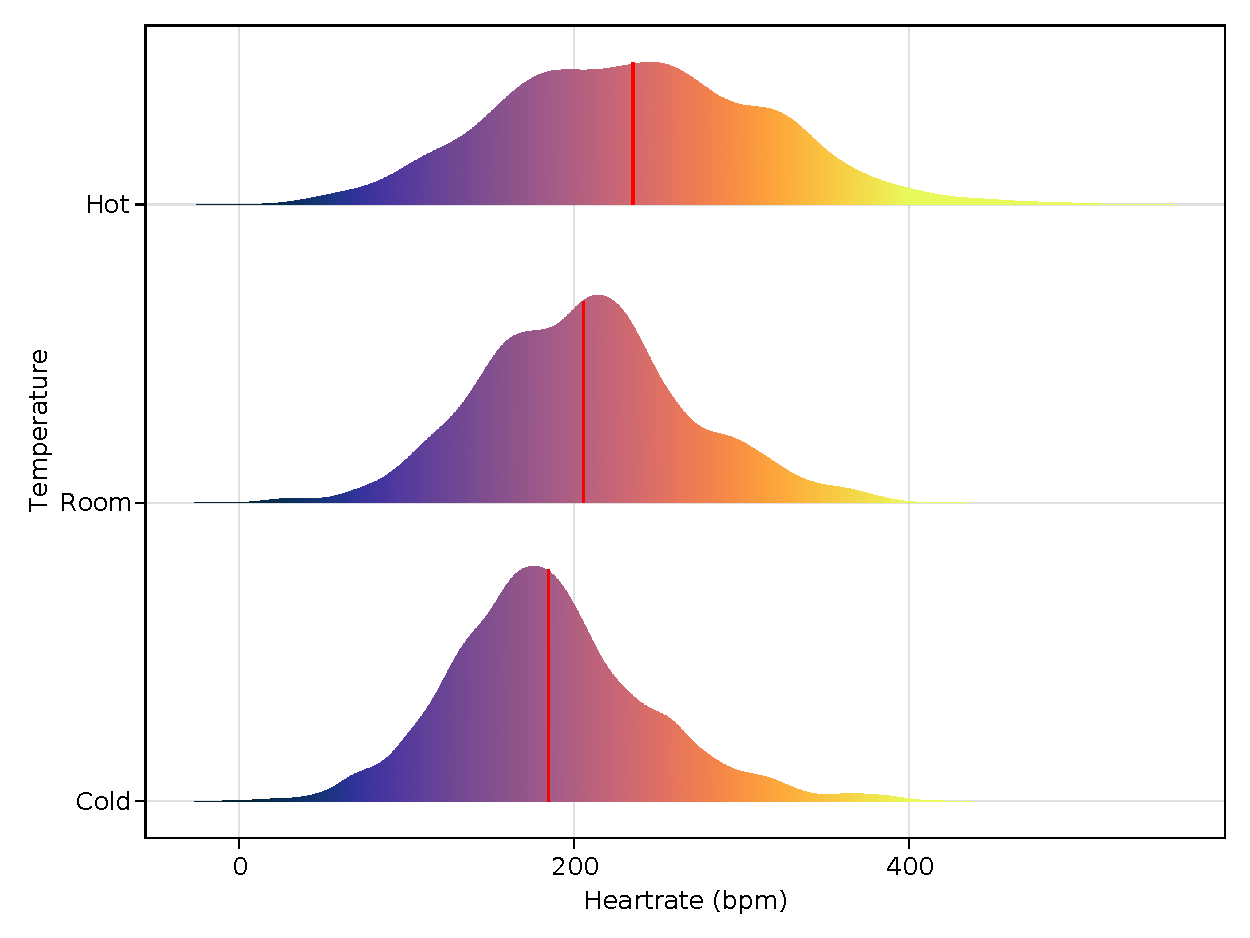
\includegraphics[width=0.75\textwidth]{figures/plot2.pdf}
    \caption{Density plot}
    \label{fig:density}
\end{figure}

% \begin{table}[ht]
% \centering
% \begin{tabular}{ |p{2cm}||p{3cm}|p{3cm}|p{2cm}|  }
%         \hline
%         \multicolumn{4}{|c|}{Supplementary data} \\
%         \hline
%         Temperature& Standard deviation & Standard error & CLM\\
%         \hline
%         Cold &58.21&1.29& 2.53\\
%         Room&61.24&1.36& 2.66\\
%         Hot &78.04&1.73&3.39\\
%         \hline
% \end{tabular}
% \caption{}
% \label{table:1}
% \end{table}

\begin{table}[htb]
    \centering
    \begin{tabular}[]{llll}
        \addlinespace
        \toprule
        Temperature& Standard deviation & Standard error & CLM\\
        \midrule
        Cold &58.21&1.29& 2.53\\
        Room&61.24&1.36& 2.66\\
        Hot &78.04&1.73&3.39\\
        \bottomrule
    \end{tabular}
    \caption{Supplementary data}
    \label{table:1}
\end{table}


\section{Discussion}

In spite of the lacking dataset, we are able to make meaningful statements. The analysis of the data presents a clear trend, the heartrate of Daphnia is highly temperature-dependant.
There is a clear correlation between ambient temperature and heartrate, and thus metabolic rate. This effect on metabolic rate has many far reaching consequences, some known, and many more not. Further research regarding the specific effects of increased metabolic rate in Daphnia and other aquatic poikilotherms is needed. These organisms play vital roles in freshwater ecosystems, that ultimately have far reaching  effects on the global ecosystem.
\printbibliography
\end{document}